%Section: "Comparison of the methods"  (JC)
%       -rate of convergence of PMFs
%       -each method's Dz with same PMF (no)
%       -each method's PMF with same Dz (no)
%       -does any method stand out?
%
%    Section: Error tolerance and robustness (Conner)
%       -modeling PMFs / D(z) using simple functions and limited data (e.g., just a couple of points along the curve)
%       -range of logP$_m$s obtained depending on uncertainty

\section{Comparison of methods and tolerance to error}
  \par Results presented up to this point do not favor any one method over another.  For example, while REMD-US is more accurate for urea, it is less so for the other two permeants (see Table~\ref{table:results}).  To examine if the rate of convergence depends on the method employed, we have plotted for each method and permeant log\perm~as a function of simulation time in Fig.~\ref{fig:deltaP}.  For codeine and benzoic acid, the variance in log\perm~for a given method is quite small, no more than 0.25 log units, even between 360\,ns and almost 3\,$\mu$s, suggesting that as much as 90\% of the simulation time invested was unnecessary.  On the other hand, there is a clear effect of time on log\perm~for urea, with it changing by as much as two log units over time.   The downward trend for urea's log\perm~is an effect of the shrinking peak in the PMF (Fig.~\ref{fig:PMFs}C).   A similar trend for codeine or benzoic acid is likely not observed because the peaks in their PMFs, i.e., those parts above 0 that contribute most significantly to log\perm, are almost non-existent.   Regardless, for codeine and benzoic acid, the disagreement with experiment is notable in part because the simulated values are consistently greater by 0.5 to 1.5 log units.

%\begin{figure}[htbp]
%\begin{center}
%	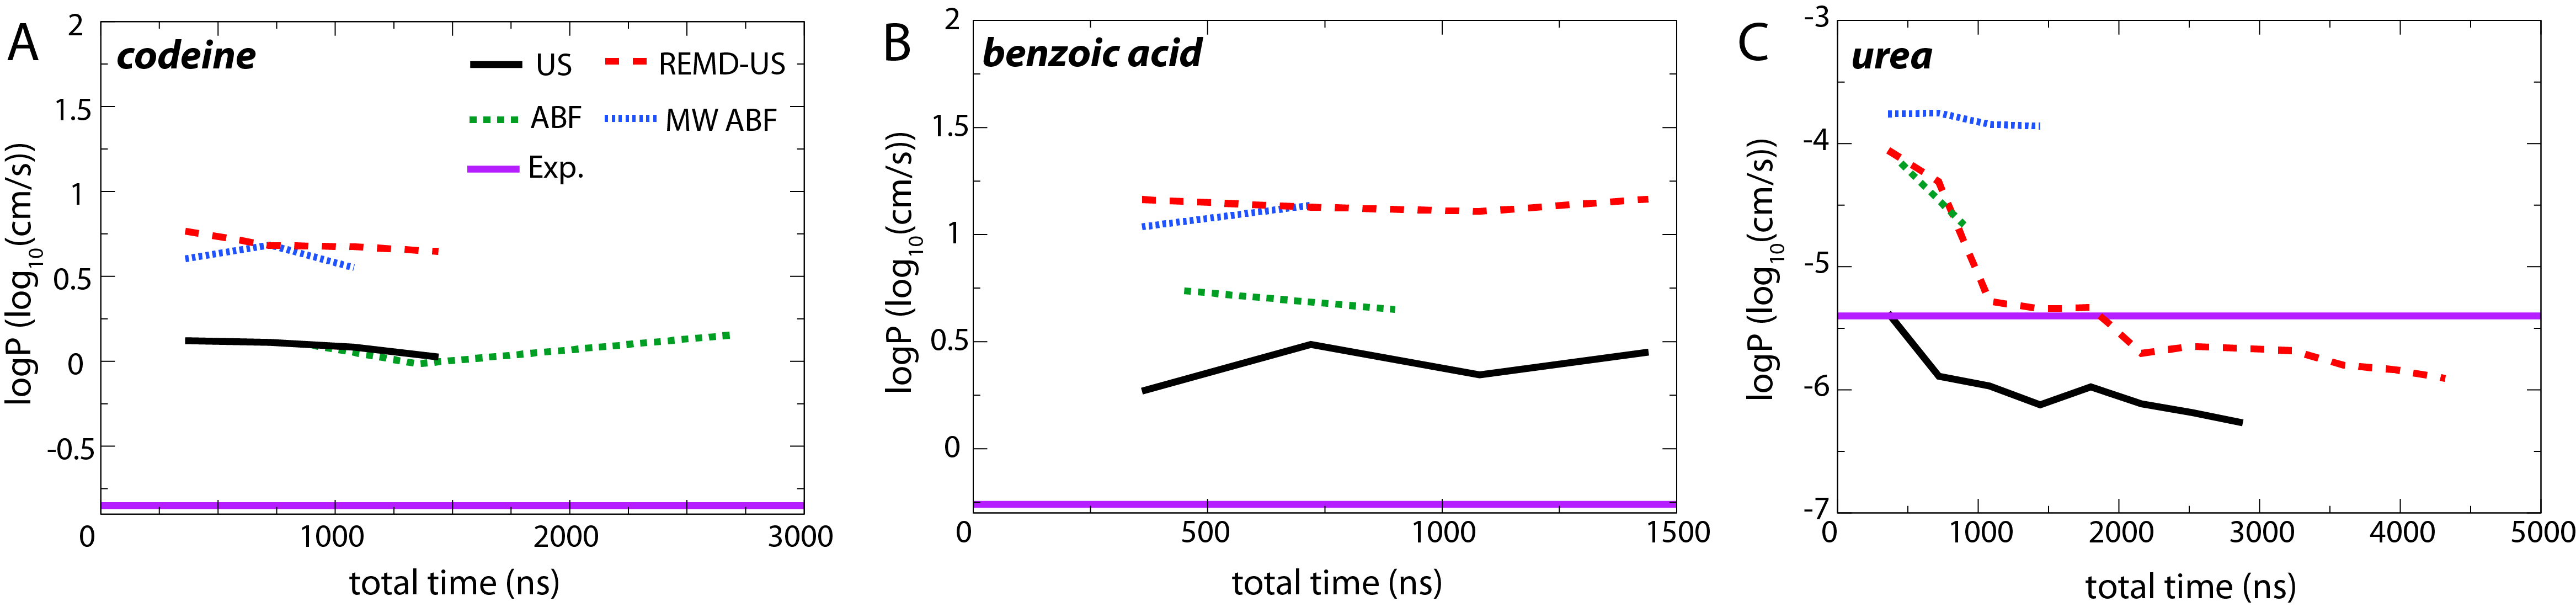
\includegraphics[width=0.9\textwidth]{Figures/converge}
%	\caption{Convergence of log\perm~for the three permeants, (A) codeine, (B) benzoic acid, and (C) urea.  Experimental values are shown as solid purple lines, with those from the simulations as indicated in the legend.}
%	\label{fig:converge}
%\end{center}
%\end{figure}

%\section*{Error tolerance}

  \par After examining the PMFs and diffusivities in great detail, it is useful to consider their individual contributions to the permeability and, thus, how accurate each of them ought to be to give log\perm~at a chosen level of accuracy.  To explore how these two parameters contribute to the permeability, a program to generate arbitrary PMFs and diffusivities was written.  This program creates smooth profiles based on input values of the PMF and diffusivity at the interfacial region and at the center of the membrane (see Methods for more details).  We first used the program to test molecules with a single barrier (or valley) at the membrane center, varying the barrier's height and width.  As seen in Fig.~\ref{fig:models}A, the contribution of the width is negligible, while the height of the barrier dominates log\perm.  For positive PMF values
  %greater than 0\,kcal/mol
 at the center, there is roughly a correspondence of 2\,kcal/mol to one log unit for log\perm.  Changing the diffusivity by a factor of 10 (range of $10^{-6}$ to $10^{-5}$\,cm$^2$/s) has a similar effect of one log unit, as expected from the linear dependence of the permeability on $D$($z$) (see Fig.~\ref{fig:models}B).  Nearly identical behavior was observed when two barriers were placed at the interfacial region, with only the height and not the position of the barriers contributing (see Fig.~S7).

\begin{figure}[htbp]
\begin{center}
	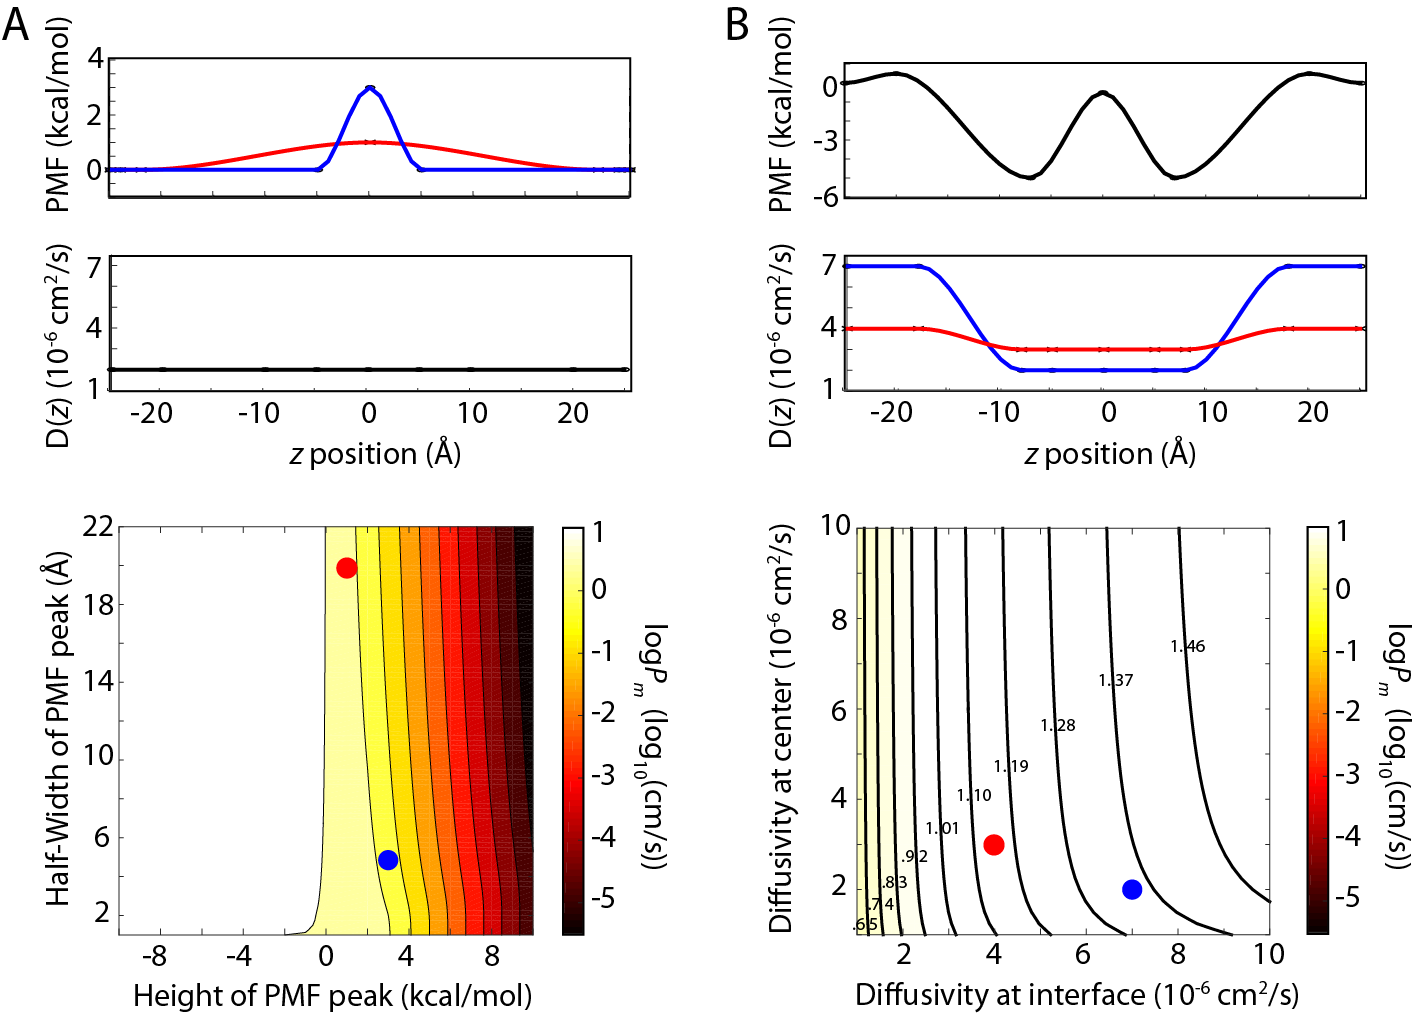
\includegraphics[width=0.9\textwidth]{Figures/models}
	\caption{log\perm~as a function of modeled input.  In both parts, the input PMF and $D$($z$) are shown on top and the dependence of log\perm~on them on bottom.  In each contour plot, the red and blue circles correspond to the red and blue PMF or diffusivity above.  (A) log\perm~as a function of PMF barrier height and width.  $D$($z$) is held constant.  (B) log\perm~as a function of diffusivity profile.  The PMF is held constant.  $D$($z$) is varied at $z=\pm 20$\,\AA~(interface) and at $z=0$\,\AA~(center).  The range of log\perm~values is 0.55 to 1.55, with contour values given in the figure.}
	\label{fig:models}
\end{center}
\end{figure}

  \par While permeants for which the PMF barrier is pronounced have their log\perm~values dominated by the barrier height, others may exhibit more subtle dependencies.  To test this possibility, a PMF in which the barriers are less than 1\,kcal/mol at the interfacial regions of the membrane, akin to the PMFs for codeine or benzoic acid, was created and the diffusivity profile varied.  As shown in Fig.~\ref{fig:models}B, the diffusivity at the PMF barriers contributes to log\perm, but that at the core (a minimum in the PMF) does not.  As a final test of the minimal amount of information necessary to calculate log\perm, we generated PMFs and diffusivities to match those from simulation based solely on the PMF value at the peak(s) and $D$($z$) at that position.  Comparison of each generated profile to the computed ones is presented in Fig.~S8.  The obtained log\perm~values are 0.31 (benzoic acid), 0.44 (codeine), and $-5.82$ (urea).  While urea is identical to the value estimated with REUS (see Table~\ref{table:results}), the other two permeants are slightly below their computed values (difference of 0.85 and 0.63, respectively), although they are closer to experimental values.  Regardless, our models demonstrate that log\perm~can be obtained from surprisingly few data points to a high degree of accuracy.

%Even so, an order of magnitude change in the diffusivity only changes the log\perm~by 1 log unit, as would be expected from the functional dependence in Eq.~\ref{eq:xx}.

%The net result of the idealized profiles is that a calculation of log\perm~is dominated by, first and foremost, the PMF maximum.  Indeed, if precision to within one log unit is all that is required, the maximum of the PMF is sufficient.  Further precision can be obtained by knowing the diffusivity at the maximum.  As evidence of this point, we determined log\perm~for each permeant using our program and only the location(s) and value(s) of the PMFs at their maxima.  ... (to do)

%Because the solubility-diffusion model relies on two position-dependent quantities, the PMF and diffusivity, it is natural to assume they must be calculated to determine the permeability.  However, as demonstrated in the section ``Comparison of methods and tolerance to error'', only a few data points contribute significantly to it.  Therefore,
  \par In lieu of determining the full PMF, which can require microseconds of simulation, one can use alternative methods to sample the critical points, i.e., at the interface and/or at the center.  As a proof-of-concept, we ran alchemical free energy perturbation (FEP) to calculate the solvation free energy of urea in the membrane core and in water.  We found $\Delta G = 9.26$\,kcal/mol ($\sim$1--1.5\,kcal/mol higher than predicted by our PMFs in Fig.~\ref{fig:PMFs}) and $D(0) = 1.25\times 10^{-6}$\,cm$^2$/s.  When combined with a very simple interpolated PMF curve that goes smoothly to 0 at $z=\pm20$\,\AA, we find log\perm = $-5.26$.  This is within < 3\% of the experimental value, despite requiring significantly less simulation time: 200\,ns for FEP vs. at least 1\,$\mu$s for the full-PMF approach.  However, one loses insight into the details of the permeation process when using FEP over a PMF-based method.


%Thus, we recommend that sampling be focused on critical regions where barriers are expected, e.g., the membrane core and/or interfacial region.
